\section{The Proposed Approach}
\label{sec:propApproach}
\subsection{Speech Signals Database}
\par To conduct this research, a series of speech signals were collected from people living in São José do Rio Preto city, state of São Paulo, Brazil. Data samples were acquired from 21 individuals, of which 20 were used since, in one case, it was not possible to get complementary information. Such recordings consist of digits, in the range from 0 to 9, spoken both in English and in Brazilian Portuguese languages. The speakers were chosen according to their gender and age so that the dataset covers people from pre-school children to adults up to 67 years old, males and females.
\\
\par The recordings were made with an Asus smartphone model \textit{Ze550kl}, running the \textit{Android 6.0.1} operating system, in different environments with various noise levels in the background, ensuring a good variability of common interference and, thus, characterizing real situations. The speech data were stored in the \textit{wave} file format with no compression, quantization of 16-bit, and a sampling rate of 44100Hz, allowing for, according to the Nyquist theorem, frequencies up to 22050Hz to be registered.
\\
\par Once the signals were collected, the spoken digits were separated one by one with a tool built in Bash script programming language, resulting in a total of 410 voice signals of different lengths that were labeled ``genuine''. For each of them, the corresponding replayed signal was created by playing and recording the original one in a silent room with an \textit{Acer} computer model \textit{Travelmate B} running the \textit{Arch GNU/Linux} operating system. That procedure produced the 410 corresponding signals we labeled as ``spoofed''.
\subsection{Database Organization}
\par The signals were sorted by type, that is, genuine or spoofed, by language, by digit that was dictated, and the interlocutor considered. A hierarchical directory structure was created to allow for an easy and intuitive access to each of the speech files, whether by automated means or not. The spoofed files reside in the ``playback'' directory, while the genuine ones are in the ``live'' directory. This organization is illustrated in Figures \ref{fig:directorystructlevel01}, \ref{fig:directorystructlevel02}, and \ref{fig:directorystructlevel03}.
\begin{figure}[ht]
\centering
\subfloat[0.33\textwidth][Database level 1]{
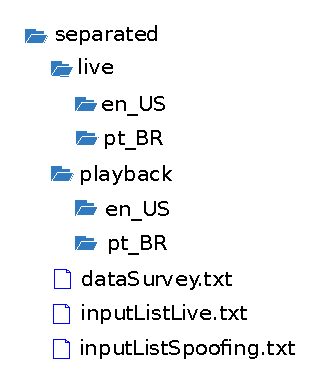
\includegraphics[height=152px]{images/directoryStructLevel01.pdf}
\label{fig:directorystructlevel01}
			}
\subfloat[0.33\textwidth][Database level 2]{
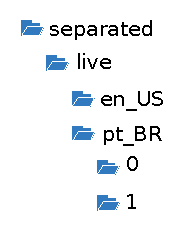
\includegraphics[height=103px]{images/directoryStructLevel02.pdf}
\label{fig:directorystructlevel02}
			}
\subfloat[0.33\textwidth][Database level 3]{
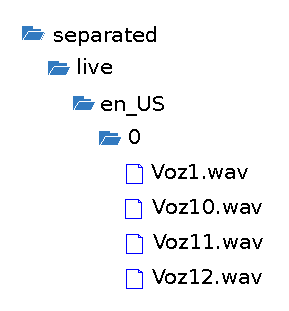
\includegraphics[height=120px]{images/directoryStructLevel03.pdf}
\label{fig:directorystructlevel03}
			}
\caption{Database organization}
\label{fig:directorystructlevel010203}
\end{figure}
\par Additional information and notes on the speech files were included in three text files, as follows:
\begin{itemize}
\item \textit{\textbf{dataSurvey.txt}}: Contains age and gender data along with a file name generated for each speaker.
\item \textit{\textbf{inputListLive.txt}}: A list of paths for all genuine files.
\item \textit{\textbf{inputListSpoofing.txt}}: A list of paths for all spoofed files.
\end{itemize}
Just as an example, the directory contents of the \textbf{``separated \textfractionsolidus live \textfractionsolidus en\_US \textfractionsolidus 0''} path consists of several \textit{wave} files, each identifying the speaker to which it belongs to, as shown in Figure \ref{fig:directorystructlevel03}. This directory contains the ``zero'', i.e., original vocalizations for digit ``zero'' from all speakers.
\subsection{Proposed Approach Structure}
\par The proposed strategy to differentiate genuine speech from the spoofed ones was designed as illustrated in Figure \ref{fig:propApproachStruct}. Overall, our technique consists in converting the raw data from all 410 + 410 = 820 genuine and spoofed voice signals to their corresponding feature vectors. Subsequently, the best feature subsets are chosen based on PFE. Proceeding, random separations were used to isolate the feature vectors destined for training/modeling from those destined for classification tests, where either a distance-based strategy or an SVM algorithm \cite{bennett2000support} was adopted. Lastly, the tests were performed and the results were registered.
\\
\par Particularly, the following sequence of steps was carried out:
\newpage
\begin{itemize}
\item{}\textbf{BEGINNING}
\item{}\textbf{STEP $S_1$: }All the 820 signals were normalized in such a way that their amplitude samples fall within the range $(-1,1)$. In addition, just the central part from each speech signal, for which the length matches the greatest power of two, was effectively considered to proceed, allowing for the wavelet transformations to be performed \cite{guidodwt1}. Then, each signal was converted to a corresponding feature vector based on the DTWPT, migrating from the time domain to the time-frequency domain. The deepest transformation level was adopted, implying a maximum frequency resolution and a minimum temporal resolution \cite{guidodwt1}. The following wavelet filters were experimented: Haar, Daubechies with support-sizes from 4 to 76, Symmlets with support-sizes 8, 16, and 32, Coiflets with support-sizes 6, 12, 18, 24, and 30, Beylkin with support-size 18, and Vaidyanathan with support-size 24. 
\item{}\textbf{STEP $S_2$: }The samples of the wavelet-transformed signals in the deepest level were grouped together to match either Bark \cite{bossi} or Mel scales \cite{bossi2} and, then, each band's normalized energy was computed \cite{tut_se}-pp.265, i.e., $$\text{i-th band's energy}=\frac{\sum\limits_{k \hspace*{+2pt} \in \hspace*{+2pt} \text{i-th band}}{{(f_k)}^{2}}}{\sum\limits_{j \hspace*{+2pt} \in \hspace*{+2pt} \text{all bands}}^{}{(f_j)}^{2}}, \qquad \text{for} \quad i=0, 1, ..., \text{number of bands}\qquad .$$ Consequently, for the former and the latter auditory scales, 24-sample long and 13-sample long feature vectors were obtained, respectively, according to their definitions \cite{bossi2} and as can be seen in the horizontal axes of Figures from \ref{fig:livehaarbark} to \ref{fig:spoofingdaub54mel}, in the next Section.  
\item{}\textbf{STEP $S_3$: }Considering the classes ``genuine'' and ``spoofed'', PFE was used to perform both intra-class and inter-class analyses, checking the particular features in the feature vectors that are most adequate to distinguish between the classes, as a function of the wavelet filter and the auditory scale. The result from a PFE analysis consists of a point $P=(G_1,G_2)$ in the paraconsistent plane, as in paper \cite{8588433}. According to PFE theory, the closer $P$ is from the corner $(1,0)$ of that plane, the better the set of features under analysis is to distinguish between the classes, as shown in Figure \ref{fig:pfe}. 
\item{}\textbf{STEP $S_4$: }Once the best features have been found, they are used in this classification step, where two strategies were tested independently: Distance-based and SVM-based. In the former, which characterizes a pattern-matching approach, Euclidian and Manhattan distances were experimented. The latter was chosen because previous studies prove its effectiveness for binary classification \cite{bennett2000support}. Different amounts of data were used for modeling/training and testing, as described in Section \ref{sec:testsResults}.
\\
\\
In particular, the three-layer SVM structure adopted, according to Figure \ref{fig:3layersSVM}, is composed of:
	\begin{itemize}
	\item{}an input passive layer, for which the dimension matches that of the feature vector selected by the PFE analysis.
	\item{}a hidden active non-linear layer, based on Radial Basis Function (RBF) kernels, for which the dimension matches the number of training feature vectors being used. 
	\item{}an output layer with one active linear element. 
    \item{}a set of weights between the input layer and the hidden layer, all of them equal the unity. 
    \item{}a set of $X$ weights, i.e., $\{p_0, p_1, ..., p_{X-1}\}$, between the hidden layer and the output layer.
    \end{itemize}
The SVM is trained by using a semi-supervised approach. First, in the non-supervised part, the $i$-th element in the hidden layer is adjusted to output the maximum value, i.e., $1$, when the $i$-th training vector is used as input. Then, during the supervised part, $\{p_0, p_1, ..., p_{X-1}\}$ are determined in an one-step strategy resulting from the solution of a linear squared system of equations\cite{poole2014linear}. The labels ``1'' and ``-1'' were used to represent genuine and spoofed speech signals, respectively.  
\item{}\textbf{END.}
\end{itemize}
\begin{figure}[h]
	\centering
	\caption{Estrutura da estratégia proposta}
	\scalebox{0.75}	{
		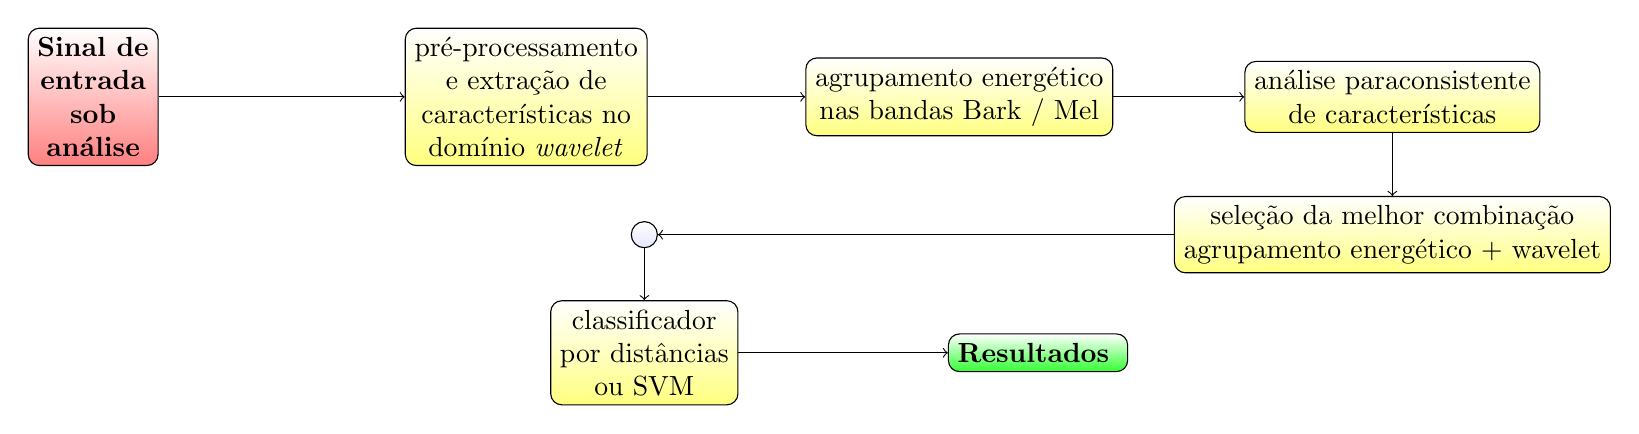
\begin{tikzpicture} 
			\node (z1)[shape=rectangle, rounded corners, draw, align=center, top color=white, bottom color=red!50] 
			at (0,2){
				\textbf{Sinal de} \\ \textbf{entrada} \\ \textbf{sob} \\ \textbf{análise}
			}; 
				
			\node (z2)[shape=rectangle, rounded corners, draw, align=center, top color=white, bottom color=yellow!50] 
			at (5.5,2){
				pré-processamento \\ e extração de \\ características no \\ domínio \textit{wavelet}
			}; 	
			
			\node (z3)[shape=rectangle, rounded corners, draw, align=center, top color=white, bottom color=yellow!50] 
			at (11,2){
				agrupamento energético \\ nas bandas Bark / Mel
			}; 	
			
			\node (z4)[shape=rectangle, rounded corners, draw, align=center, top color=white, bottom color=yellow!50] 
			at (16.5,2){
				análise paraconsistente \\ de características
			}; 
			
			\node (z5)[shape=rectangle, rounded corners, draw, align=center, top color=white, bottom color=yellow!50] 
			at (16.5,0.25){
				seleção da melhor combinação \\ agrupamento energético + wavelet
			}; 
					
			\node (z6)[shape=circle, draw, align=center, top color=white, bottom color=blue!10] 
			at (7,0.25) {};
			
			\node (z7)[shape=rectangle, rounded corners, draw, align=center, top color=white, bottom color=yellow!50] 
			at (7,-1.25) {
				classificador \\ por distâncias \\ ou SVM
			};
			
			\node (z8)[shape=rectangle, rounded corners, draw, align=center, top color=white, bottom color=green!80] 
			at (12,-1.25) {
				\textbf{Resultados}
			};
			
			\path[->] (z1) edge (z2);
			\path[->] (z2) edge (z3);
			\path[->] (z3) edge (z4);
			\path[->] (z4) edge (z5);
			\path[->] (z5) edge (z6);
			\path[->] (z6) edge (z7);	
			\path[->] (z7) edge (z8);
		\end{tikzpicture}
	}
	\label{fig_arq}
	\\Fonte: Elaborado pelo autor, 2021.
\end{figure}
\begin{figure}
	\centering
	\scalebox{2}{
				\begin{tikzpicture}
	%input layer
	\node (input1) at (0.65,2.0) {};
	\draw[->,in=180,out=0] (1.0,2.0) to (1.35,2.0);
	\node (input2) at (0.65,1.5) {};
	\draw[->,in=180,out=0] (1.0,1.5) to (1.35,1.5);
	\node (input3) at (0.65,1.0) {};
	\draw[->,in=180,out=0] (1.0,1.0) to (1.35,1.0);
	\node (input3) at (0.65,0.0) {};
	\draw[->,in=180,out=0] (1.0,0.0) to (1.35,0.0);
	\node (IL_N1) at (1.5,2.0) {}; \filldraw[fill=gray!30] (1.5,2.0) circle (0.15cm);
	\node (IL_N2) at (1.5,1.5) {}; \filldraw[fill=gray!30] (1.5,1.5) circle (0.15cm);
	\node (IL_N3) at (1.5,1.0) {}; \filldraw[fill=gray!30] (1.5,1.0) circle (0.15cm);
	\node at (1.5,0.625) {$\vdots$};
	\node (IL_Nn) at (1.5,0.0) {}; \filldraw[fill=gray!30] (1.5,0.0) circle (0.15cm);
	
	%hidden layer 
	\node (HL_N1) at (3.5,2.5) {}; \filldraw[fill=blue!20] (3.55,2.5) circle (0.15cm);
	\node (HL_N2) at (3.5,2.0) {}; \filldraw[fill=blue!20] (3.55,2.0) circle (0.15cm);
	\node (HL_N3) at (3.5,1.5) {}; \filldraw[fill=blue!20] (3.55,1.5) circle (0.15cm);
	\node (HL_N4) at (3.5,1.0) {}; \filldraw[fill=blue!20] (3.55,1.0) circle (0.15cm);
	\node at (3.55,0.625) {$\vdots$};
	\node (HL_Nn-1) at (3.5,0.0) {}; \filldraw[fill=blue!20] (3.55,0.0) circle (0.15cm);	
	\node (HL_Nn) at (3.5,-0.5) {}; \filldraw[fill=blue!20] (3.55,-0.5) circle (0.15cm);	
	\draw[->,in=180,out=0] (IL_N1)+(1.5mm,0) to (HL_N1);
	\draw[->,in=180,out=0] (IL_N1)+(1.5mm,0) to (HL_N2);
	\draw[->,in=180,out=0] (IL_N1)+(1.5mm,0) to (HL_N3);
	\draw[->,in=180,out=0] (IL_N1)+(1.5mm,0) to (HL_N4);
	\draw[->,in=180,out=0] (IL_N1)+(1.5mm,0) to (HL_Nn-1);
	\draw[->,in=180,out=0] (IL_N1)+(1.5mm,0) to (HL_Nn);
	
	\draw[->,in=180,out=0] (IL_N2)+(1.5mm,0) to (HL_N1);
	\draw[->,in=180,out=0] (IL_N2)+(1.5mm,0) to (HL_N2);
	\draw[->,in=180,out=0] (IL_N2)+(1.5mm,0) to (HL_N3);
	\draw[->,in=180,out=0] (IL_N2)+(1.5mm,0) to (HL_N4);
	\draw[->,in=180,out=0] (IL_N2)+(1.5mm,0) to (HL_Nn-1);
	\draw[->,in=180,out=0] (IL_N2)+(1.5mm,0) to (HL_Nn);
	
	\draw[->,in=180,out=0] (IL_N3)+(1.5mm,0) to (HL_N1);
	\draw[->,in=180,out=0] (IL_N3)+(1.5mm,0) to (HL_N2);
	\draw[->,in=180,out=0] (IL_N3)+(1.5mm,0) to (HL_N3);
	\draw[->,in=180,out=0] (IL_N3)+(1.5mm,0) to (HL_N4);
	\draw[->,in=180,out=0] (IL_N3)+(1.5mm,0) to (HL_Nn-1);
	\draw[->,in=180,out=0] (IL_N3)+(1.5mm,0) to (HL_Nn);
	
	\draw[->,in=180,out=0] (IL_Nn)+(1.5mm,0) to (HL_N1);
	\draw[->,in=180,out=0] (IL_Nn)+(1.5mm,0) to (HL_N2);
	\draw[->,in=180,out=0] (IL_Nn)+(1.5mm,0) to (HL_N3);
	\draw[->,in=180,out=0] (IL_Nn)+(1.5mm,0) to (HL_N4);
	\draw[->,in=180,out=0] (IL_Nn)+(1.5mm,0) to (HL_Nn-1);
	\draw[->,in=180,out=0] (IL_Nn)+(1.5mm,0) to (HL_Nn);
	
	%output layer
	\node (OL_N1) at (5.5,1.0) {}; \filldraw[fill=red!40] (5.55,1.0) circle (0.15cm);
	
	\draw[->,in=180,out=0] (HL_N1)+(2mm,0) to (OL_N1);
	\draw[->,in=180,out=0] (HL_N2)+(2mm,0) to (OL_N1);
	\draw[->,in=180,out=0] (HL_N3)+(2mm,0) to (OL_N1);
	\draw[->,in=180,out=0] (HL_N4)+(2mm,0) to (OL_N1);
	\draw[->,in=180,out=0] (HL_Nn-1)+(2mm,0) to (OL_N1);
	\draw[->,in=180,out=0] (HL_Nn)+(2mm,0) to (OL_N1);
	%
	\draw[snake=brace,mirror snake,raise snake=45pt,brown] (1.25,1.25) -- (1.75,1.25) node[black,midway,yshift=-50pt,below]{\tiny camada de} node[black,midway,yshift=-58pt,below]{\tiny entrada com} node[black,midway,yshift=-66pt,below]{\tiny $R$ elementos}
	node[black,midway,yshift=-74pt,below]{\tiny passivos};
	\draw[snake=brace,mirror snake,raise snake=45pt,brown] (3.25,0.75) -- (3.75,0.75) node[black,midway,yshift=-50pt,below]{\tiny camada} node[black,midway,yshift=-58pt,below]{\tiny intermediária} node[black,midway,yshift=-66pt,below]{\tiny com $X$ neurônios}
	node[black,midway,yshift=-74pt,below]{\tiny ativos não-lineares};
	\draw[snake=brace,mirror snake,raise snake=45pt,brown] (5.25,1.75) -- (5.75,1.75) node[black,midway,yshift=-50pt,below]{\tiny camada de} node[black,midway,yshift=-58pt,below]{\tiny saída com} node[black,midway,yshift=-66pt,below]{\tiny um elemento}
	node[black,midway,yshift=-74pt,below]{\tiny ativo linear};
	%
	\node (OUT) at (6.5,1.0) {\tiny resultado}; 
	\draw[->,in=180,out=0] (OL_N1)+(2mm,0) to (OUT);	
	
	\node at (4,2.6) {\tiny $p_0$}; 
	\node at (4,2.1) {\tiny $p_1$}; 
	\node at (4,1.65) {\tiny $p_2$}; 
	\node at (4,1.2) {\tiny $p_3$}; 
	\node at (4,0.2) {\tiny $p_{X-2}$}; 
	\node at (4,-0.3) {\tiny $p_{X-1}$}; 
\end{tikzpicture}
	}
	\caption{Estrutura da SVM para o procedimento 03 com $R$ neurônios na camada de entrada, sendo $R$ a dimensão dos vetores de características, e $X$ neurônios na camada intermediária, sendo $X$ o número de casos de treinamento}
	\label{fig:3layersSVM}
\end{figure} 
\begin{figure}[H]
\centering
	\scalebox{1.5}
	{
	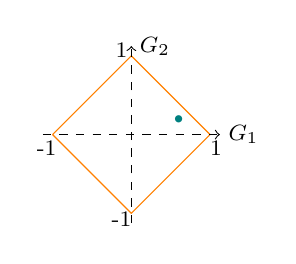
\begin{tikzpicture} 
	\draw[color=orange] (-1,0)--(0,1)--(1,0)--(0,-1)--(-1,0); 	
	\draw[dashed,color=black,->] (-1.125,0)--(1.125,0) node{\footnotesize \qquad $G_1$}; 	
	\draw[dashed,color=black,->] (0,-1.125)--(0,1.125) node{\footnotesize \qquad $G_2$}; 
	\node at (-1.075,-0.175){\footnotesize -1};	
	\node at (1.075,-0.175){\footnotesize 1};	
	\node at (-0.125,1.075){\footnotesize 1};	
	\node at (-0.125,-1.075){\footnotesize -1};	
	\node at (0.675-0.075,+0.25-0.075){\Huge{\textcolor{teal}{$\cdot$}}};	
	\end{tikzpicture}	
	}
\caption{the paraconsistent plan derived from PFE theory. The axes, i.e., $G_1$ and $G_2$, correspond to the degrees of certainty and contradiction, respectively. Particularly, $P=(G_1,G_2)=(\alpha-\beta,\alpha+\beta-1)$, which was drawn in teal just to exemplify, is the focus of PFE analysis: the closer it is to the corner $(1,0)$ of the plane, the better the features are to distinguish between the classes and, consequently, the weaker the classifier used in conjunction with them can be. The specific values used for $\alpha$ and $\beta$ come from intra-class and inter-class analyses, respectively, as described in paper \cite{8588433}.}
\label{fig:pfe}
\end{figure} 
